\documentclass[12pt]{article}

\usepackage{graphicx}      % Enable graphics commands
\usepackage{lscape}    	% Enable landscape with \begin{landscape} until \end{landscape}
\usepackage[section]{placeins} % Keep tables and figures within their own sections
\usepackage{natbib}			% Enable citation commands \citep{}, \citet{}, etc.
\bibpunct{(}{)}{;}{a}{}{,}		% Formatting for in-text citations
\usepackage{setspace}		% Enable double-spacing with \begin{spacing}{2} until \end{spacing}.
\usepackage[utf8]{inputenc} 	% Enable utf8 characters, i.e., accents without coding--just type them in.
\usepackage[english]{babel}	% English hyphenation and alphabetization.  Other languages available.
\usepackage{dcolumn}        % For decimal-aligned stargazer output.
\usepackage[colorlinks=true, urlcolor=blue, citecolor=black, linkcolor=black]{hyperref} % Include hyperlinks with the \url and \href commands.
\setlength{\tabcolsep}{1pt}	% Make tables slightly narrower by reducing space between columns.

\renewcommand\floatpagefraction{.9}	% These commands allow larger tables and graphics to fit
\renewcommand\topfraction{.9}		% on a page when default settings would complain.
\renewcommand\bottomfraction{.9}
\renewcommand\textfraction{.1}
\setcounter{totalnumber}{50}
\setcounter{topnumber}{50}
\setcounter{bottomnumber}{50}

\newcommand{\R}{\textsf{R}~}        %This creates the command \R to typeset the name R correctly.

%\usepackage[left=1in, right=1in]{geometry}	%Turn footnotes into endnotes (commented out).
%\renewcommand{\footnotesize}{\normalsize}	
%\usepackage{endnotes}
%\renewcommand{\footnote}{\endnote}
%\renewcommand{\section}{\subsection}
%\usepackage{fullpage}

\begin{document}


\title{Protect Yourself from \emph{p}-Hacking:\\ 7 Things to Do to\\ Avoid Committing Scientific Malpractice}		
\author{
    Frederick Solt\\
    \href{mailto:frederick-solt@uiowa.edu}{frederick-solt@uiowa.edu}
    \and
    Yue Hu\\
    \href{mailto:yue-hu@uiowa.edu}{yue-hu@uiowa.edu}
    \and
	Kevan Hudson\\
	\href{mailto:kevan-hudson@uiowa.edu}{kevan-hudson@uiowa.edu}
	\and
	Jungmin Song\\
    \href{mailto:jungmin-song@uiowa.edu}{jungmin-song@uiowa.edu}
	\and
	Dong `Erico' Yu\\
    \href{mailto:dong-yu@uiowa.edu}{dong-yu@uiowa.edu}
}
\date{\today}				
\maketitle

\begin{abstract}

\end{abstract}
\newpage

% Build on the outline below.  Cite by using \citep{Author2016} to add a
% parenthetical citation; use \citet{Author2016} to get a textual cite like
% this: Author (2016). 

Replication crisis

LaCour scandal

p-Hacking.  check out special issue on p-hacking: \url{http://www.tandfonline.com/toc/hcms20/9/4}

malpractice not always so blatent or intentional: confirmation bias, garden of forking paths (see \url{http://www.stat.columbia.edu/~gelman/research/unpublished/p_hacking.pdf})

Introduce \citet{Newman2015}, perhaps noting the press attention it has received (e.g., \url{http://www.psmag.com/health-and-behavior/five-studies-bernie-sanders-says-the-rich-are-deranged})

Data Access and Research Transparency (DA-RT): A Joint Statement by Political Science Journal Editors: \url{http://journals.cambridge.org/action/displayAbstract?fromPage=online&aid=9911378&fulltextType=LT&fileId=S2049847015000448}

Sound research is a cornerstone of the advancement of knowledge across all fields of study. The need for carefully conducted, replicable empirical research is not a new concern, though it has gained additional attention of late. One instance that highlights the growing concern about research practices is the so-called replication crisis. Uncovered by the Open Science Collaboration (2015), the replication crisis highlights the severity of the problem. Of 100 published studies that the authors attempted to replicate, just 36 produced the same results as those cited in the published articles (Open Science Collaboration, 2015). Additionally cases such as that of Michael LaCour, the UCLA grad student who fabricated data, provide further proof of the need for vigilance in combatting academic fraud. Given the pressure to produce publishable work, careful consideration of how to detect and minimize academic fraud, along with processes to avoid engaging in questionable research practices are of the utmost importance.

It is important to note that academic misconduct and faulty research need not be the product of an intentional attempt to dupe the system. Confirmation bias, a well-documented tendency to accept those pieces of evidence that confirm our pre-existing beliefs while discounting evidence that counters them undoubtedly can contribute to questionable research practices. Results that support a carefully crafted theory may be accepted as robust, even without thorough examination, while those results that disconfirm the same theory may be dismissed as misspecification. Even the process of developing a model aimed at testing a theory might contribute to faulty research. Gelman and Loken’s analogy of a garden of forking paths (2013) suggests that even when researchers are not actively engaged in fishing for results, decisions that are made about how to carry out the research necessarily preclude other comparisons from being considered

Our aim in this paper is to provide a guide to avoiding in academic malpractice, a series of steps that if followed, are sure to produce sound results that are replicable and transparent, a goal that if accepted widely across academia, could minimize the occurrence of academic fraud, and halt the replication crisis in its tracks. In order to demonstrate the importance of these steps, and how issues can arise when they are ignored, we utilize a recently published article, “False Consciousness or Class Awareness? Local Income Inequality, Personal Economic Position, and Belief in American Meritocracy” by Newman et al (2015).

This article, published in the American Journal of Political Science examines the effect of local inequality on individual’s belief in the meritocratic nature of America. The findings suggest that rich and poor respond differently to local inequality, with the rich being no less likely to reject meritocracy when inequality is high, while higher inequality increases the likelihood the poor will reject meritocracy. Seen as providing further evidence of the growing gulf between the rich and poor, not just in terms of economic resources, but in their perceptions of the system they cohabitate, the results have gained media attention beyond the field of political science, being featured in a Pacific Standard article.

However, a careful consideration of the methods employed by the authors and the results they produce raise serious doubts about the soundness of the research practices the authors employed. In addressing these doubts, Newman et al (2015) provides a cautionary tale that highlights seven steps that can help researchers to avoid committing academic malpractice, both of the unintentional and intentional sort. Below we outline each of these seven steps (ADD LIST OF STEPS) and rely on Newman et al (2015) to provide illustrations of the dangers of not following these research practices.



% How does the context of income inequality affect political and economic attitudes?  Many studies have found that greater inequality tends to be associated with attitudes that reinforce rather than challenge the status quo. \citet{Newman2015}, however, argue that inequality instead activates disillusionment with the dominant U.S. ideology, leading poorer individuals in local contexts of higher inequality to become more class conscious and to reject meritocracy.  However, the article's empirical results are misinterpreted, and efforts to replicate its analyses reveal additional problems.  As a result, its sanguine conclusions regarding the prospects for redistribution are unsupported.
					% Kevan
% Build on the outline below.  Cite by using \citep{Author2016} to add a
% parenthetical citation; use \citet{Author2016} to get a textual cite like
% this: Author (2016). 

\section{Ensure Reproducibility}

Ensure Reproducibility

What is reproducibility? Reproducibility means that Researcher B obtains exactly the same results that were originally reported by Researcher A (e.g. the author of that paper) from A’s data when following the same methodology (Brunswik 1955; Asendorpf et al. 2013). 
Also, even for replicability, this paper is problematic. Replicability means that the finding can be obtained with other random samples drawn from a different time point or a different situation. As we will show as follows, they employed one survey that can strengthen their arguments and did not try to test whether their findings can be generalized to other time points and other situations. 

Why reproducibility is important.
How the present social science could develop so far based on the replication work. Examples.
Using multiple measures for the dependent variable. 

Reproducibility as bare minimum for replication; DA-RT APSA guidelines

script all work

packrat and checkpoint packages in R; version command in Stata

quote \citet{Newman2015} replication materials

Table 1 and 2 cannot be reproduced exactly

Table 3 cannot be reproduced at all: more parameters than observations
		% Jungmin
% Replace 'text' below with your text.  Use \citep{Author2016} to add a
% parenthetical citation; use \citet{Author2016} to get a textual cite like
% this: Author (2016).  FS will add the code to insert figures.

\section{Work in Public}

discuss preregistration

Github as complement

obviously \citet{Newman2015} didn't do this
				% Hu
% Build on the outline below.  Cite by using \citep{Author2016} to add a
% parenthetical citation; use \citet{Author2016} to get a textual cite like
% this: Author (2016). 

\section{Examine All Available Data}

examine as much relevant evidence as possible

discuss Figure \ref{F:t2_pooled}

discuss Figure \ref{F:t2_by_survey}

An important step in the process of conducting sound research is striving to utilize all available data. Researchers should seek to conduct their analysis on the entirety of data that they have at their disposal. Doing so provides a number of benefits:  it increases the likelihood that the sample utilized captures the true distribution of the underlying population, and it affords greater leverage in testing the implications of one’s hypothesis. While the issue of selection bias cannot be avoided simply by including all available data, limiting analysis to a particular dataset, particularly when alternatives are available, may cast doubt on the inferences drawn from that analysis. By including all relevant data researchers are better able to observe the implications of their theory, thus providing greater support for the hypotheses they advance.

If research is limited to a particular source of data, the findings may be called into question. The limited data may provide evidence of a relationship that is not present in a larger, more representative sample. We can draw an example of the dangers of not including all relevant data from \citet{Newman2015}.  In an attempt to test some underlying assumptions of their theory the authors rely on 2006 Pew Research Center dataset due to its “unique set of questions tapping perceptions of economic hierarchy and inequality and respondents perception of their own position within such a hierarchy” \citep{Newman2015 p.336}. As presented by the authors, this dataset provides the only source of information on responses to the question whether or not an American thinks of America as being divided into haves and have-nots, and whether they think of themselves as being haves or have-nots. Employing this dataset the authors find further support for their theory, in situations of higher inequality respondents are more likely to believe that America is divided in such a way, and the poor are more likely to identify themselves as have-nots. In reality, these questions are not unique to the 2006 dataset, but are instead present in each of the surveys the authors used in their earlier analysis. Perhaps it is by coincidence that, as shown in Figure \ref{F:t2_by_survey}, the coefficient of interest only achieves statistical significance when using the 2006 data. As illustrated, no other dataset produces a statistically significant coefficient for Gini according to the authors’ model. This provides a clear illustration of the importance of including all relevant data; failure to do so can lead to biased results.

The authors’ use of this severely truncated data has implications beyond the coefficient of interest as well. While Figure (INSERT FIGURE NUMBER) clearly demonstrates that a more careful inclusion of all data produce results that run counter to the findings of Newman et al, including all available data drastically changes the entre model, not merely the coefficient for Gini. Figure \ref{F:t2_pooled} provides estimates of the coefficients from Newman et al’s Table 2 (p. 336) with a sample that includes data from the 2005, 2006, 2007, and 2009 surveys they use earlier in their article. When all relevant data is included, the results are drastically different. Not only does the primary variable of interest (Gini coefficient) lose statistical significance, but others do as well. Having voted for Bush is no longer a statistically significant predictor of believing America is divided into the haves and have-nots, but income becomes strongly negative and significantly associated with the same belief. Additionally, union membership gains statistical significance, indicating that belonging to a union increases the likelihood an individual perceives that have/have-not division. Ultimately, Figure (INSERT NUMBER) provides graphical representation of the dangers of not including all available data. By limiting their analysis to the sole dataset that produced a statistically significant coefficient for inequality, the authors have disguised the true relationship in order to support their theory. A properly crafted analysis reveals findings that are far less surprising; the wealthy are less likely to see America as divided into the haves and have-nots, while union members are more likely to do so. These findings counter the primary argument advanced by Newman et al, and lend strong evidence to the claim that “we should be willing to take whatever information we can acquire so long as it helps us learn about the veracity of our theory,” while illustrating the pitfall of picking and choosing data that confirm our theory, while ignoring data that does not \citep{King1994 p.31}.


\begin{figure}[htbp] 
  \caption{Local Inequality and the Perception of America as Divided into `Haves' and `Have-Nots': Results Using All Available Data}
  \label{F:t2_pooled}
  \begin{center}
    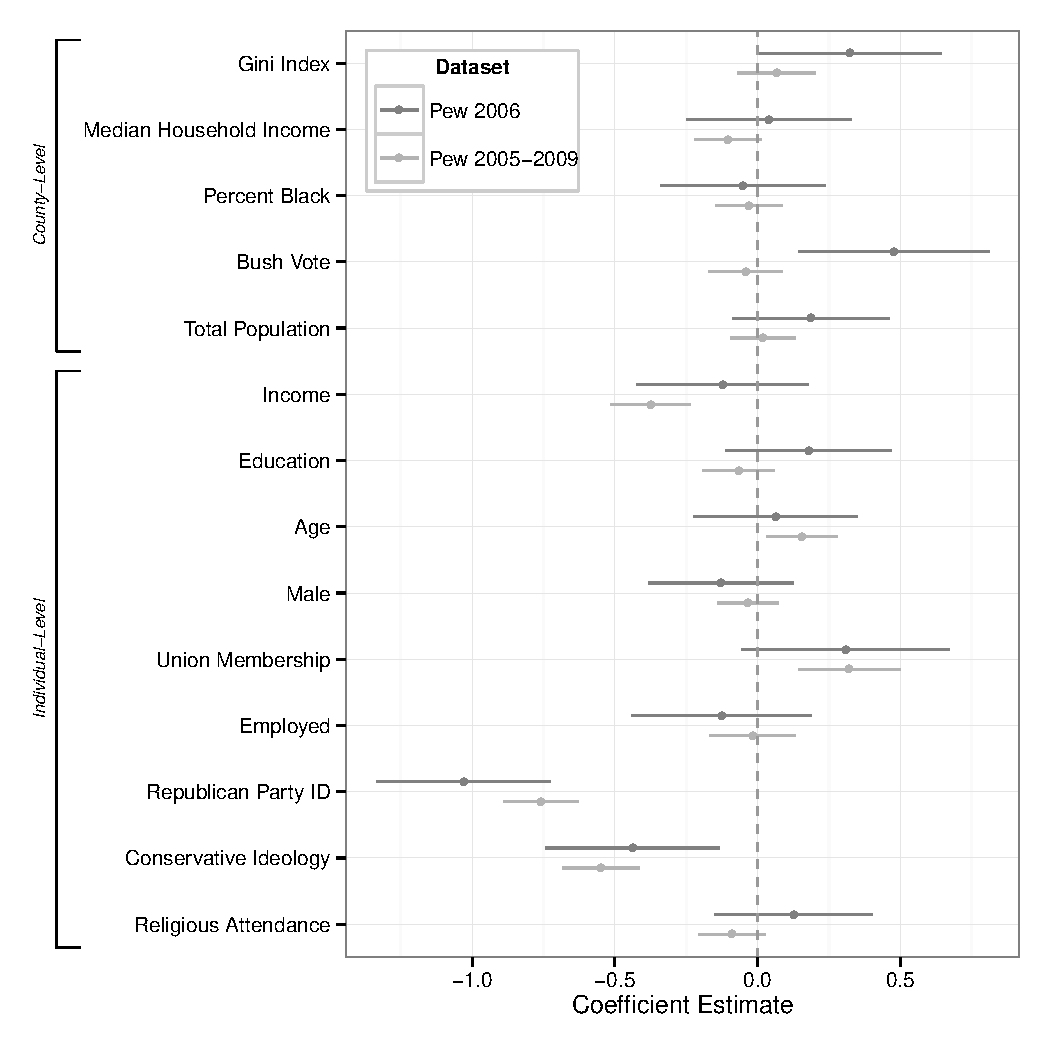
\includegraphics[width=5.25in]{../figures/03_examine_all_available_data_t2.pdf}
  \end{center}
  \begin{footnotesize}
  \begin{tabular}{p{.1in} p{5.1in}}
  & \emph{Notes}: Results from replications of the model presented in Table 2 of \citet{Newman2015} on the 2006 Pew survey analyzed in that article and on pooled data from the six Pew surveys that included the same item and were conducted in the time period the article examines.  The statistically significant result for county income inequality in the 2006 survey presented in that article is not evident when all of the available data are examined.
  \end{tabular}
  \end{footnotesize}
\end{figure}

\begin{figure}[htbp] 
  \caption{Local Inequality and the Perception of America as Divided into `Haves' and `Have-Nots': Results Using Each Available Dataset}
  \label{F:t2_by_survey}
  \begin{center}
    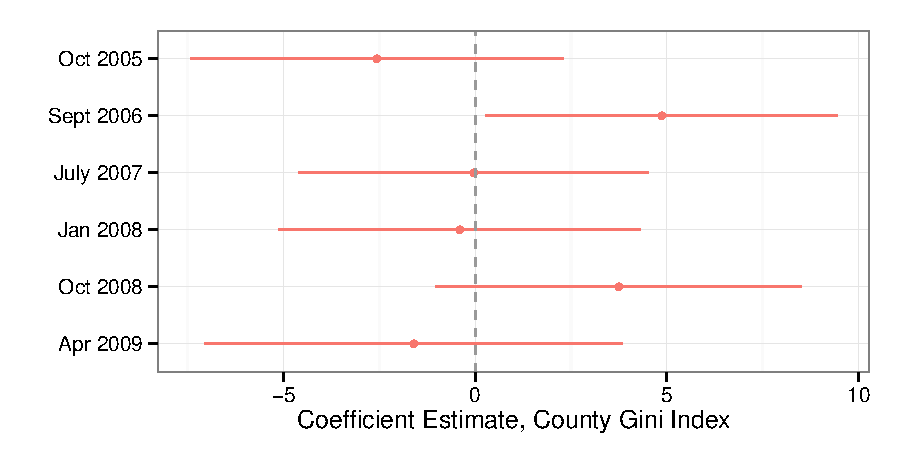
\includegraphics[width=5.25in]{../figures/03_examine_all_available_data_t2_by_survey.pdf}
  \end{center}
  \begin{footnotesize}
  \begin{tabular}{p{.1in} p{5.1in}}
  & \emph{Notes}: Results for county income inequality from replications of the model presented in Table 2 of \citet{Newman2015} on data from each of six available surveys conducted in the in the time period examined in that article.  Of the six surveys, the only one that yields a statistically significant result is the 2006 survey presented in the article.
  \end{tabular}
  \end{footnotesize}
\end{figure}



	% Kevan
% Replace 'text' below with your text.  Use \citep{Author2016} to add a
% parenthetical citation; use \citet{Author2016} to get a textual cite like
% this: Author (2016).  FS will add the code to insert figures.

\section{Use Consistent Measures}

\begin{figure}[htbp] 
  \caption{Comparing Three Measures of Rejection of Meritocracy Pooled by \citet{Newman2015} in Pew Surveys, 1999-2012}
  \label{F:three_measures}
  \begin{center}
    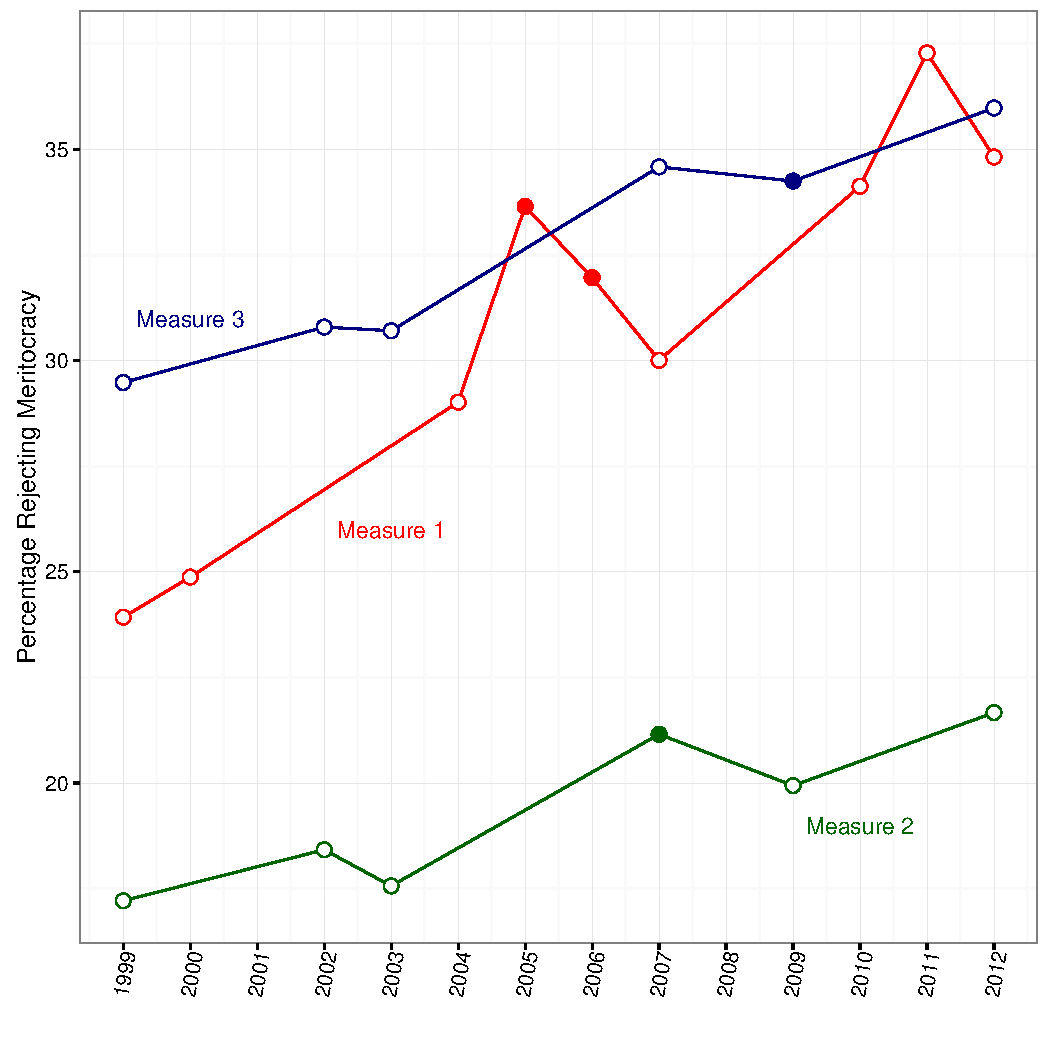
\includegraphics[width=5.25in]{../figures/04_three_measures_dv.pdf}
  \end{center}
  \begin{footnotesize}
  \begin{tabular}{p{.1in} p{5.1in}}
  & \emph{Notes}: The analyses presented in Table 1 of \citet[333]{Newman2015} were conducted on pooled observations with the dependent variable, rejection of meritocracy, measured in one of three different ways \citep[see][331]{Newman2015}.  Plotting the percentage of (weighted) respondents to reject meritocracy by each of these measures in various Pew surveys reveals that the second measure results in much lower levels of rejection of meritocracy than either of the others and the third often yields considerably higher levels than the first.  In light of the evident lack of comparability of these three measures, pooling them into a single analysis cannot be justified.
  \end{tabular}
  \end{footnotesize}
\end{figure}

		% Hu
% Build on the outline below.  Cite by using \citep{Author2016} to add a
% parenthetical citation; use \citet{Author2016} to get a textual cite like
% this: Author (2016). 


\section{Handle Data with Care}

need to be really careful: double-check!  Also need to be transparent.

merging: data on Bush share of vote don't match

input{../figures/05_handle_data_with_care_bush_al.tex}

coding and recoding: NJL's five point party id scale collapses leaners and weak partisans (not weak and strong partisans, and not leaners and `true' independents).  Should really use the full seven point scale; no reason to throw away that information (or to deviate from common practice)

unemployment is mismeasured in 2005, 2007, and 2009 in Table 1 due to missing employ2 variable---all of those who are not working (students, retired, etc.) are coded as unemployed
				% Erico
% Build on the outline below.  Cite by using \citep{Author2016} to add a
% parenthetical citation; use \citet{Author2016} to get a textual cite like
% this: Author (2016). 

\section{Multiply Impute Missing Data}

Summary Paragraph\par

In political science study, a common way to contaminate the data and undermine the validity is missing data growing non-response in Pew survey (Curtain, et.al, 2005;);\par

Reason: poor survey design(literature needed); private information (income;  ); sensitive question—influence of social desiablity (underreported abortion of black: Jagannathan, 2001; nonrespond and overreponse in female president question; Streb, 2008; nonresponse in religious: Hadway et.al, 1993); survey forms (Chang RDDv.s. Internet; 2009; Amazon-Turk, Berinsky, 2012)\par

To deal with missing data: first identify missing mechanisms: (1) missing completely at random (MCAR): the probability of missingness is the same for all unit; that is, each survey respondent choose not to answer the question based on on coin flip (2)missing at random (MAR), and nonignorable or (King et. al, 2001): the probability whether the survey question is answered may depend on the other factor which are observable in the data: for example, an independents are more tend to decline to answer partisan identification question. (3)nonignorable (NI): because of the unobserved value of the missing response: high income people tend to conceal their real income, and other variables in the data cannot predict which respondent have high income.\par

Strategy: to all: 1. listwise deletion or complete-case analysis; +  Available case study  (use the distribution of other observable variables)\par

Disadvantages: (1) lead to biased estimates, especially when missing values differ systematically from the completed observed cases; (2) relatively, the standard error can be sensitive due to the original sample size and the deleted case size; (3) in ACS, may lead to omission of a variable hat is necessary to satisfying the assumptions necessary for desired casual inference.\par

2. Non-response weighting: need to add literatures (for MAR and MCAR)\par

3. Simple imputation: With high certainty: (1 )mean, (2)last value carried forward;\par

With uncertainty: (3) using information from related observation (for example, in GSS, using reported occupation types and its mean annual salary to infer income; or in SIS, use reported working months to infer income)\par
 
Disadvantages:  (1) mean, last value, or other singly imputed method bias, especially when the size of missing observation is relatively large; distorting the actual distribution (Gelman, 2006)\par

(2) Inferred from other related observation: may not to impute all missing data\par

4. Random Imputation with a single variable or multiple variables\par

5. Multiple Imputation:\par

Definition: imputing missing values for each missing case with different imputations to reflect uncertainty levels, and creating a complete data set. (King.et.al, 2001). For example, if assume the missing data of a specific variable is MAR, indicating other observable variables can infer useful information to predict the missing cases,  conditional on whichever imputation model adopted.\par

(1)Multivariate regression:\par
a. use continuous model to impute missing discrete response.Example: modeling the data as continuous (transfer discrete value into continuous), and imputing continuous values (Gelman and King, 1998) \par

(2)

Specific to Newman’s paper\par
church attendance---all missing are simply assigned ``once or twice a month"

income, a variable of interest, is missing for over 10\% of the sample, but values are mysteriously single-imputed (where did these values come from? they aren't meaningful--they fall between categories)

ideology, partyid also single-imputed, it seems

Church attendance: MAR

income: MAR

ideology: MAR

Thus, mulitple imputation is possible and necessary

missing data should be multiply imputed \citep[e.g.,][]{King2001}



				% Erico

It has been well known for over a decade that models containing multiplicative interaction terms require particular care in interpretation \citep[see, e.g.,][]{Golder2003a, Braumoeller2004, Brambor2006, Kam2007a}

\begin{figure}[htbp] 
  \caption{Logit Coefficients of Local Income Inequality by Respondent Income: Table 1, Model 1, From Replication Data}
  \label{F:coef.t1m1}
  \begin{center}
    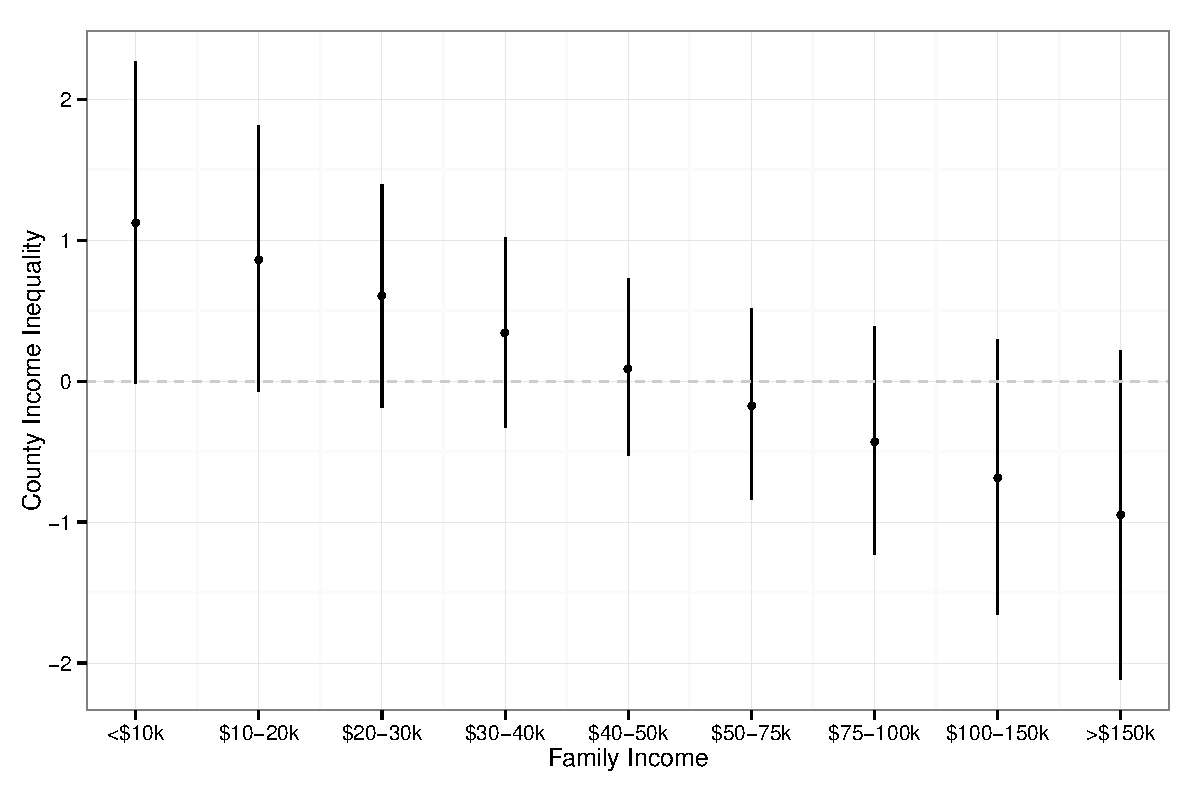
\includegraphics[width=5.25in]{../figures/07_plot_interaction_terms_t1m1.pdf}
  \end{center}
  \begin{footnotesize}
  \begin{tabular}{p{.1in} p{5.1in}}
  & \emph{Notes}: The coefficient for county income inequality fails to reach statistical significance for any observed level of respondent family income.
  \end{tabular}
  \end{footnotesize}
\end{figure}


% \begin{figure}[htbp] 
%   \caption{Logit Coefficients of Local Income Inequality by Respondent Income, Table B1, White Respondents, From Source Data}
%   \label{F:coef.b1m1}
%   \begin{center}
%     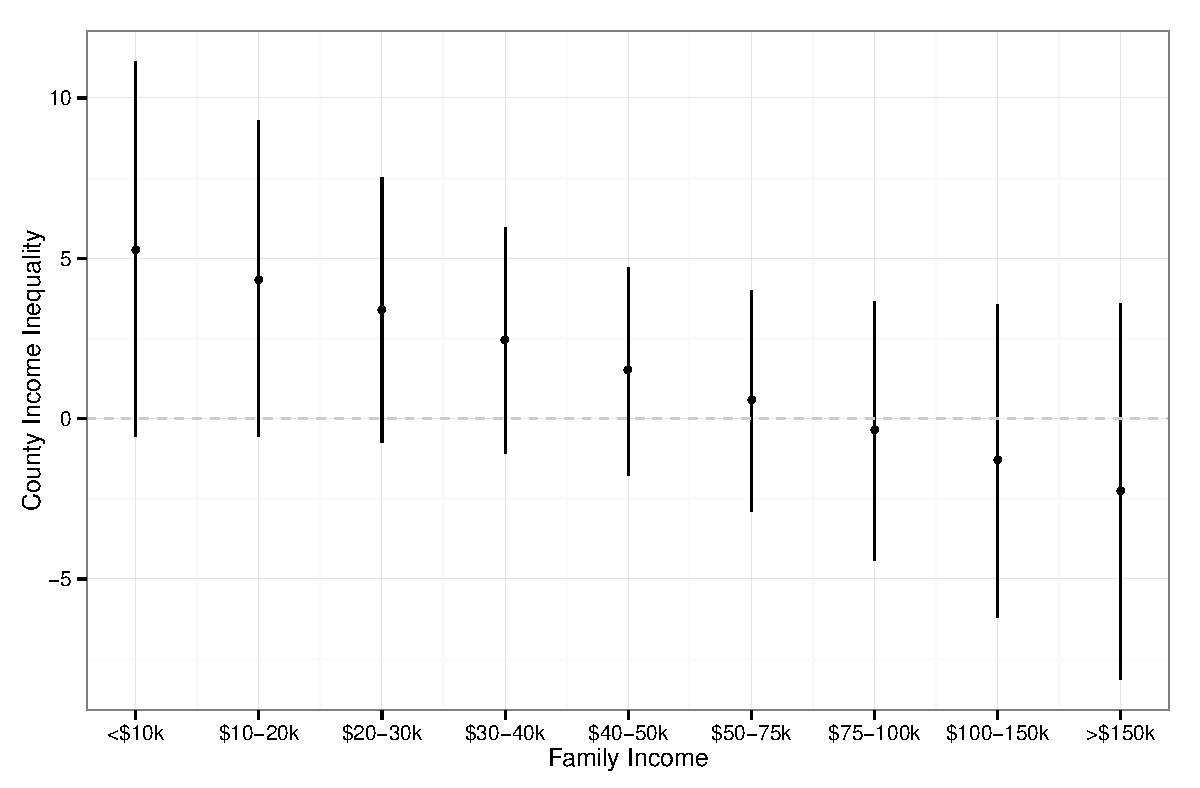
\includegraphics[width=5.25in]{b1m1_mi_plot.pdf}
%   \end{center}
%   \begin{footnotesize}
%   \begin{tabular}{p{.1in} p{5.1in}}
%   & \emph{Notes}: The coefficient for county income inequality fails to reach statistical significance for any observed level of respondent family income.
%   \end{tabular}
%   \end{footnotesize}
% \end{figure}

		% Jungmin

% \input{10_introduction_example}
% \input{11_ensure_reproducibility_example}
% \input{12_code_in_public_example}
% \input{13_examine_all_available_data_example}
% \input{14_use_consistent_measures_example}
% \input{15_recode_with_care_example}
% \input{16_multiply_impute_example}
% \input{17_plot_interaction_terms_example}

\newpage
\pagebreak

\bibliographystyle{bib/ajps}
\bibliography{bib/avoid}

\end{document}